The result of Fermat's Farctorization method factorizing a set of growing primes as seen in \ref{numbersuites}.


\begin{figure}[H]
\centering
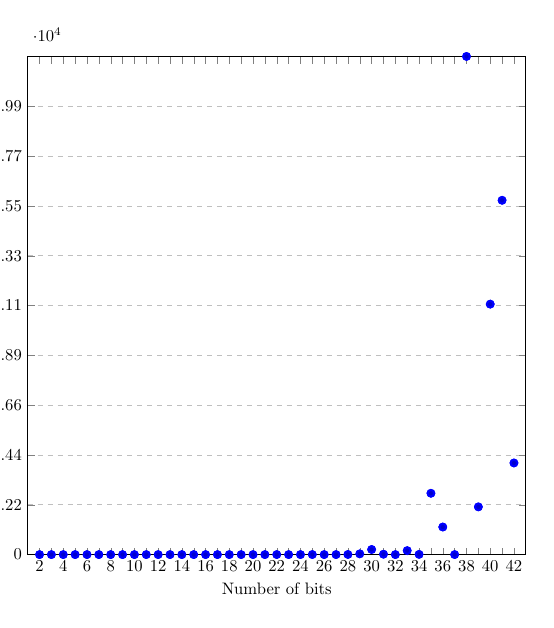
\begin{tikzpicture}[scale=0.6, trim axis left, trim axis right]
\begin{axis}[
    width=1\textwidth,
    height=1\textwidth,
    xlabel={Number of bits},
    ylabel={Time taken (s)},
    xmin=1.0, xmax=43.0,
    ymin=7e-06, ymax=22132.913785,
    xticklabels={2, , 4, , 6, , 8, , 10, , 12, , 14, , 16, , 18, , 20, , 22, , 24, , 26, , 28, , 30, , 32, , 34, , 36, , 38, , 40, , 42},
    xtick={2, 3, 4, 5, 6, 7, 8, 9, 10, 11, 12, 13, 14, 15, 16, 17, 18, 19, 20, 21, 22, 23, 24, 25, 26, 27, 28, 29, 30, 31, 32, 33, 34, 35, 36, 37, 38, 39, 40, 41, 42},
    ytick={7e-06, 2213.2913848, 4426.5827626, 6639.8741404, 8853.1655182, 11066.456896, 13279.7482738, 15493.0396516, 17706.3310294, 19919.6224072},
    ymajorgrids=true,
    grid style=dashed,
]

\addplot+[
    blue,
    very thick,
    forget plot,
    only marks
    ]
    plot[
    very thick,
    error bars/.cd,
    y dir=plus,
    y explicit
    ]
    table[x=x,y=y,y error expr=\thisrow{y-max}] {
    x    y    y-max
    28	5.8406775	0.0704825
24	1.7399245	0.0221965
25	3.6471474	0.0090486
26	0.1470242	0.0007868
27	0.0866493	0.0006217
20	0.0158812	0.0001738
21	0.0031789	4.81e-05
22	1.5685366	0.0389564
23	0.0608879	0.0011291
42	4071.78641	0.0
29	33.1152222	0.0806078
40	11128.625773	0.0
41	15742.323432	0.0
3	1.32e-05	1.8e-06
2	9.6e-06	1.14e-05
5	1.32e-05	8e-07
4	1.35e-05	5.5e-06
7	1.22e-05	8e-07
6	1.23e-05	7e-07
9	1.22e-05	8e-07
8	1.29e-05	1e-07
13	0.0003992	1.38e-05
12	0.0002527	1.43e-05
11	1.22e-05	8e-07
10	2.14e-05	1.06e-05
39	2120.144309	0.0
38	22132.913785	0.0
15	4.31e-05	9e-07
14	0.0001948	2.2e-06
17	0.0017258	2.22e-05
16	3.43e-05	7e-07
19	0.0086429	3.71e-05
18	0.0548063	0.0012267
31	17.4857932	0.0410988
30	227.2125548	0.6077562
37	1.1880925	0.0020695
36	1225.201901	2.305899
35	2724.45897	0.405076
34	10.1863916	0.0999634
33	176.7157063	0.5127967
32	0.004257	3.8e-05

    };

\addplot+[
    blue,
    very thick,
    forget plot,
    only marks
    ]
    plot[
    very thick,
    error bars/.cd,
    y dir=plus,
    y explicit
    ]
    table[x=x,y=y,y error expr=\thisrow{y-min}] {
    x    y    y-min
    28	5.8406775	-0.0253155
24	1.7399245	-0.0109965
25	3.6471474	-0.0155404
26	0.1470242	-0.0004742
27	0.0866493	-0.0010043
20	0.0158812	-9.02e-05
21	0.0031789	-2.59e-05
22	1.5685366	-0.0140606
23	0.0608879	-0.0003739
42	4071.78641	0.0
29	33.1152222	-0.0618232
40	11128.625773	0.0
41	15742.323432	0.0
3	1.32e-05	-1.2e-06
2	9.6e-06	-2.6e-06
5	1.32e-05	-2e-07
4	1.35e-05	-1.5e-06
7	1.22e-05	-2e-07
6	1.23e-05	-3e-07
9	1.22e-05	-2e-07
8	1.29e-05	-9e-07
13	0.0003992	-4.2e-06
12	0.0002527	-4.7e-06
11	1.22e-05	-2e-07
10	2.14e-05	-1.4e-06
39	2120.144309	0.0
38	22132.913785	0.0
15	4.31e-05	-1e-07
14	0.0001948	-1.8e-06
17	0.0017258	-1.68e-05
16	3.43e-05	-3e-07
19	0.0086429	-5.59e-05
18	0.0548063	-0.0004313
31	17.4857932	-0.0380652
30	227.2125548	-0.4542478
37	1.1880925	-0.0020695
36	1225.201901	-2.305899
35	2724.45897	-0.405076
34	10.1863916	-0.0342876
33	176.7157063	-0.5290123
32	0.004257	-3.2e-05

    };

\end{axis}
\end{tikzpicture}
\vspace{-0.3cm}
\caption{Fermats Factorization Growing primes }\label{fig:FermatsFactorizationGrowing}
\end{figure}


The factorization went well until it starts to factorize a whole number consisting of two 35 bits long prime numbers. From this point it starts to take a large amount of time to factorize. After the whole number, consisting of two 42 bits worth of prime numbers, the algorithm was stopped because the factorization did not finish within eight hours. 
More Fermat's plots can be found in the appendix.